\chapter{Vita}

% Change the descriptions accordingly

%\foreach \n in {1,...,\numberOfAuthors}{
\vfill


\includegraphics[width=0.2\columnwidth]{pv}
\documentAuthor{firstname1} \ \documentAuthor{surname1} is currently pursuing Bachelor of Science Degree in Computer Engineering at De La Salle University-Manila. His role in the group is the Domain Expert. Along with his extensive ability in correlating needed topics in specifying both the strengths and projected weaknesses of the project, he contributes mainly in creating the knowledge pool of the group.

\vfill
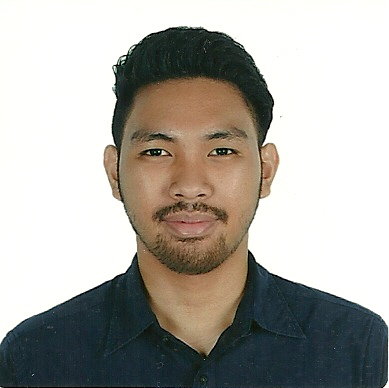
\includegraphics[width=0.2\columnwidth]{dan}
\documentAuthor{firstname2} \ \documentAuthor{surname2} is currently pursuing Bachelor of Science Degree in Computer Engineering at De La Salle University-Manila. His role in the group is the Master Programmer. With his adept skills in computer programming, he functions as the brain of the project, as he provides the main idea along with its purpose it serves. His research interests include mountaineering, agriculture, and robotics.

\vfill
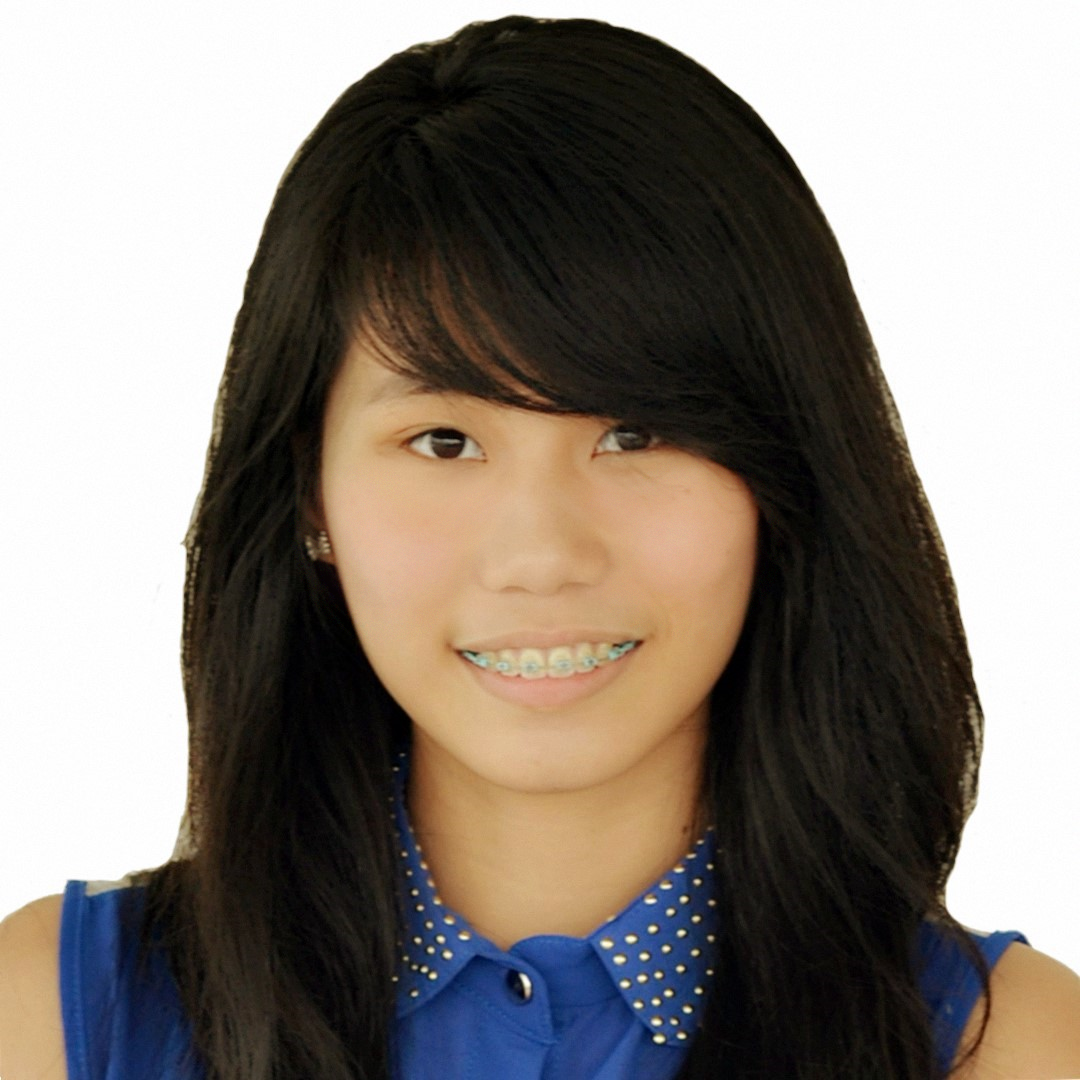
\includegraphics[width=0.2\columnwidth]{kath}
\documentAuthor{firstname3} \ \documentAuthor{surname3} is currently pursuing Bachelor of Science Degree in Computer Engineering at De La Salle University-Manila. With her keen sight for details, she provides constructive criticisms as to where the group will set rooms for further improvements and necessary corrections from established ideas. Her research interest include biomedical engineering, nanotechnology, and energy management systems.




\vfill
%}